\documentclass{standalone}
\usepackage[utf8x]{inputenc}
\usepackage{tikz}
% \usepackage{pgfplots,pgfplotstable}
\usepackage{color}

\usetikzlibrary{arrows,positioning} 
\definecolor{myorange}{RGB}{230,97,1}
\definecolor{mylightorange}{RGB}{253,184,99}
\definecolor{mypurple}{RGB}{94,60,153}
\definecolor{mylightpurple}{RGB}{178,171,210}
\definecolor{mycolor1}{RGB}{35,139,69}
\definecolor{mycolor2}{RGB}{102,194,164}
\definecolor{mycolor3}{RGB}{178,226,226}
\definecolor{mycolor4}{RGB}{237,248,251}

\begin{document}

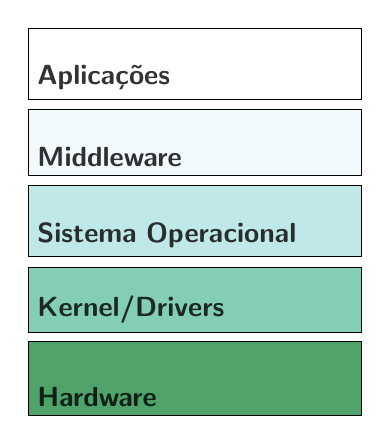
\begin{tikzpicture}[font=\sffamily]
      \begin{scope}[shift={(0cm,0cm)}, fill opacity=0.8]
        \node[draw,text width=4cm,text height=0.6cm] 
        at (0,0) {\textbf{Aplicações}};
        \node[draw,text width=4cm,text height=0.6cm, fill=mycolor4] 
        at (0,-1) {\textbf{Middleware}};
        \node[draw,text width=4cm,text height=0.6cm, fill=mycolor3] 
        at (0,-2) {\textbf{Sistema Operacional}};
        \node[draw,text width=4cm,text height=0.5cm, fill=mycolor2] 
        at (0,-3) {\textbf{Kernel/Drivers}};
        \node[draw,text width=4cm,text height=0.7cm, fill=mycolor1] 
        at (0,-4) {\textbf{Hardware}};
      \end{scope}
\end{tikzpicture} 

\end{document}
